\documentclass{article}

\usepackage{graphicx}
\graphicspath{ {./images/} }
\usepackage{amsthm}
\usepackage{amsfonts}
\usepackage{amsmath}
\usepackage{amssymb}
\usepackage{fullpage}
\usepackage[usenames]{color}
\usepackage{hyperref}
  \hypersetup{
    colorlinks = true,
    urlcolor = blue,       % color of external links using \href
    linkcolor= blue,       % color of internal links 
    citecolor= blue,       % color of links to bibliography
    filecolor= blue,        % color of file links
    }
    
\usepackage{listings}

\definecolor{dkgreen}{rgb}{0,0.6,0}
\definecolor{gray}{rgb}{0.5,0.5,0.5}
\definecolor{mauve}{rgb}{0.58,0,0.82}

\lstset{frame=tb,
  language=haskell,
  aboveskip=3mm,
  belowskip=3mm,
  showstringspaces=false,
  columns=flexible,
  basicstyle={\small\ttfamily},
  numbers=none,
  numberstyle=\tiny\color{gray},
  keywordstyle=\color{blue},
  commentstyle=\color{dkgreen},
  stringstyle=\color{mauve},
  breaklines=true,
  breakatwhitespace=true,
  tabsize=3
}

\theoremstyle{theorem} 
   \newtheorem{theorem}{Theorem}[section]
   \newtheorem{corollary}[theorem]{Corollary}
   \newtheorem{lemma}[theorem]{Lemma}
   \newtheorem{proposition}[theorem]{Proposition}
\theoremstyle{definition}
   \newtheorem{definition}[theorem]{Definition}
   \newtheorem{example}[theorem]{Example}
\theoremstyle{remark}    
  \newtheorem{remark}[theorem]{Remark}


\title{CPSC-354 Report}
\author{Keoni Lanoza  \\ Chapman University}

\date{\today}

\begin{document}

\maketitle

\begin{abstract}
Short  summary of purpose and content.  
\end{abstract}

\tableofcontents

\section{Introduction}\label{intro}

\begin{verbatim}
Name: Keoni Lanoza
Class: Programming Languages
Section: CPSC354-01
Email: lanoza@chapman.edu
\end{verbatim}

This document is a collection of homework assignment answers as requested by Prof. Kurz. This report will replace a generic midterm and final exam and will be thought of as a take home exam to be worked on throughout the semester in addition to a final project.



\section{Homework}\label{homework}

This section will contain your solutions to homework.
For every week, you will have a subsection that contains your answers.

\subsection{Week 1}

\begin{verbatim}
print("Please enter integer A")
aString = input("a: ")
while True:
    try: 
        a = int(aString)
        break
    except ValueError:
        print("Not an integer. Please try again.")
        print("Please enter INTEGER A")
        aString = input("a: ")
    
print("Please enter integer B")
bString = input("b: ")
while True:
    try: 
        b = int(bString)
        break
    except ValueError:
        print("Not an integer. Please try again.")
        print("Please enter INTEGER B")
        bString = input("b: ")

a = int(aString)
b = int(bString)

while (a != b):
    if (a > b):
        a = a - b
    elif (b > a):
        b = b - a
        
print ("The greatest common divisor is: " + str(a))
\end{verbatim}

\indent
This program works by first asking the user to input an integer named "A". 
The program stores this input in a variable called "aString" and then utilizes error checking to make sure the user's input can be converted into an integer.
If the input cannot be converted into an integer, the program loops until the user enters valid input.
If the user's input passes error checking, the program then prompts the user for an integer named "B" and follows the same error-checking process.
Once the user passes error checking for both variables, the program enters a loop.
In the loop, if integer A is greater than integer B, then integer A is replaced with the value of integer A - integer B.
If integer B is greater than integer A, then integer B is replaced with the value of integer B - integer A.
This process repeats until integer A is equal to integer B. When this is reached, the greatest common divisor of the original integer A and original integer B is printed out to the user.

For example, if we took A to be an integer representing the value of 9, and B to be an integer representing the value of 33, the program would follow this process:
Because B, which equals 33 is greater than A, which equals 9. B's value would be replaced with B - A, which is 24. B is still greater than A, so B's value would be replaced by B - A again which now equals 15.
15 is still greater than 9, so B would become 6. Now, A with a value of 9 is greater than B which has a value of 6. A would be replaced with A - B which equals 3. This makes B greater than A again.
B is now replaced with B - A, or 6 - 3, which equals 3. Now that A and B are equal, the greatest common divisor, which is 3 because both A and B equal 3, is output to the user.

\subsection{Week 2}

\begin{verbatim}
import Data.List
import System.IO

select_evens :: [Int] -> [Int]
select_evens (x:xs) = [(x:xs)!!y | y <- (y:ys)] 
  where (y:ys) = [1,3..(length (x:xs)-1)]

select_odds :: [Int] -> [Int]
select_odds (x:xs) = [(x:xs)!!y | y <- (y:ys)] 
  where (y:ys) = [0,2..(length (x:xs)-1)]

member :: Int -> [Int] -> Bool
member _ _ = False
member x (y:ys)
  | x == y = True
  | otherwise = member x ys

append :: [Int] -> [Int] -> [Int]
append (x:xs) (y:ys) = x:xs ++ y:ys

revert :: [Int] -> [Int]
revert [] = []
revert (x:xs) = revert (xs) ++ [x]

less_equal :: [Int] -> [Int] -> Bool
less_equal (x:xs) (y:ys)
  | x >= y = False
  | length (xs) == 0 && length (ys) == 0 = True
  | otherwise = less_equal xs ys

Select_Evens Computation:
select_evens [1,2,3,4,5] =
[] : [(1,2,3,4,5)!!1 | 1 <- ([1,3]) =
2 : [(1,2,3,4,5)!!3 | 3 <- ([1,3]) =
[2, 4]

Select_Odds Computation:
select_odds [1,2,3,4,5] =
[] : [1,2,3,4,5)!!0 | 0 <- ([0,2,4]) =
1 : [(1,2,3,4,5)!!2 | 2 <- ([2,4]) =
1 : (3 : [(1,2,3,4,5)!!4 | 4 <- ([4]) =
[1,3,5] 

Member Computation:
member 1 [3, 2, 1] =
1 == 3 = False, so member 1 [2,1] =
1 == 2 = False, so member 1 [1] =
1 == 1 = True, so 1 is a member of [3, 2, 1]

Append Computation:
append [1,2] [3,4,5] =
1 : (append [2] [3,4,5]) =
1 : (2 : (append [] [3,4,5]) =
1: (2: [3,4,5]) =
[1,2,3,4,5]

Revert Computation:
revert [1,2,3,4,5] =
append (revert [2,3,4,5]) ([1]) =
append (append (revert [3,4,5]) ([2])) ([1]) =
append (append (append (revert [4,5]) ([3])) ([2])) ([1]) =
append (append (append (append (revert [5]) ([4])) ([3])) ([2])) ([1]) =
append (append (append (append (append (revert []) ([5])) ([4])) ([3])) ([2])) ([1]) =
append (append (append (append (append [] ([5])) ([4])) ([3])) ([2])) ([1]) =
append (append (append (append (append [] ([5])) ([4])) ([3])) ([2])) ([1]) =
append (append (append (append ([5]) ([4])) ([3])) ([2])) ([1]) =
append (append (append ([5,4]) ([3])) ([2])) ([1]) =
append (append ([5,4,3]) ([2])) ([1]) =
append ([5,4,3,2]) ([1]) =
[5,4,3,2,1]

Less_Equal Computation:
less_equal [1,2,3] [2,3,4] =
1 >= 2 = False, so less_equal [2,3] [3,4] =
2 >= 3 = False, so less_equal [3] [4] =
3 >= 4 = False, so less_equal [] [] =
True


\end{verbatim}

\subsection{Week 3}

\begin{verbatim}
Tower Of Hanoi correct computations for a tower of 5
hanoi 5 0 2
  hanoi 4 0 1 
    hanoi 3 0 2
      hanoi 2 0 1 
        hanoi 1 0 2 = move 0 2 
        move  0 1
        hanoi 1 2 1 = move 2 1 
      move 0 2  
      hanoi 2 1 2  
        hanoi 1 1 0 = move 1 0  
        move  1 2  
        hanoi 1 0 2 = move 0 2 
    move 0 1
    hanoi 3 2 1
      hanoi 2 2 0
        hanoi 1 2 1 = move 2 1
        move 2 0
        hanoi 1 1 0 = move 1 0
      move 2 1
      hanoi 2 0 1
        hanoi 1 0 2 = move 0 2
        move 0 1
        hanoi 1 2 1 = move 2 1
  move 0 2
  hanoi 4 1 2
    hanoi 3 1 0
      hanoi 2 1 2
        hanoi 1 1 0 = move 1 0
        move 1 2
        hanoi 1 0 2 = move 0 2
      move 1 0
      hanoi 2 2 0
        hanoi 1 2 1 = move 2 1
        move 2 0
        hanoi 1 1 0 = move 1 0
    move 1 2
    hanoi 3 0 2
      hanoi 2 0 1
        hanoi 1 0 2 = move 0 2
        move 0 1
        hanoi 1 2 1 = move 2 1
      move 0 2
      hanoi 2 1 2
        hanoi 1 1 0 = move 1 0
        move 1 2
        hanoi 1 0 2 = move 0 2

\end{verbatim}

Hanoi appears in the computation 31 times.
We can express the number of times "hanoi" appears for any number n of disks with the formula: 

\begin{math}
$$numHanoi =2^{numDisks}-1$$
\end{math}

\subsection{Week 4}
\begin{verbatim}
Concrete Syntax Trees

1. 2+1
           Exp
         /       \
       Exp  +   Exp1
        |        |
      Num        Num
        |          |
        2          1

2. 1+2*3
           Exp
         /       \
       Exp  +   Exp1
        |          |
      Num          Exp1
        |          /   \
        1        Exp1 * Exp2
                   |       |
                 Num      Num
                  |         |
                  2         3 

3. 1+(2*3)
           Exp
         /       \
       Exp  +   Exp2
        |          |
      Num        ( Exp 1 )
        |          /   \
        1        Exp1 * Exp2
                   |       |
                 Num      Num
                  |         |
                  2         3 

4. (1+2)*3
           Exp1
         /       \
       (Exp)  *   Exp2
      /       \      |
    Exp  +  Exp1     Num
      |      |        |
      Num   Num       3
      |       |
      1       2      

5. 1+2*3+4*5+6
                  Exp
               /       \
            Exp    +     Exp1
            /                 \
         Exp                       Exp
        /     \                /         \ 
      Num       Exp1            Exp1        Num 
       |      /      \         /      \       |
       1    Exp1 * Exp2       Exp1 *  Exp2    6
              |       |        |        |
             Num   Num       Num       Num
              |        |        |        |
             2         3       4         5

Abstract Syntax Trees

1. 2+1
        +
      /    \
     2      1

2. 1+2*3
             +
           /   \
          1     *
              /    \
             2      3

3. 1+(2*3) (Same as 2 because parantheses are not in the grammar)
             +
           /   \
          1     *
              /    \
             2      3

4. (1+2)*3 (Same as 2 because parantheses are not in the grammar)
             +
           /   \
          1     *
              /    \
             2      3        

5. 1+2*3+4*5+6
                  +
            /          \
          +             +
       /     \       /      \
     1       *        *      6
           /   \    /  \ 
          2    3    4  5


\end{verbatim}

\subsection {Week 5}
\begin{verbatim}
1. x
EVar
  |
Ident
  |
  x

2. x x
EApp
|    \
EVar  EVar
|       |
Ident   Ident
|       |
x       x

3. x y
EApp
|    \
EVar  EVar
|       |
Ident   Ident
|       |
x       y

4. x y z
EApp
|    \
EApp  EVar
|   \     \
EVar  EVar Ident
|       |     |
Ident Ident   z
|       |
x       y

5. \ x.x
EAbs
|    \
Ident EVar
|      |
x      Ident
        |
        x

6, \ x.x x
EAbs
|    \
Ident EApp
|     |   \
x    Evar   Evar
      |     |
      x     x

7. (\ x . (\ y . x y)) (\ x.x) z
EApp
|      \
EApp      EVar
|      \          \
EAbs      EAbs       Ident
|     \    \    \           \
Ident  EAbs Ident EVar        z
|       |   \    \    \
x       y   EApp  x   Ident
             |  \         \
             EVar  EVar     x
             |       |
             Ident Ident
             |       |
             x       y

8. (\ x . (\ y . x y)) (\ x.x) z
EApp
|   -------------------\
EApp                 EVar
|   ---------\          -----------\
EApp         EVar                  Ident
|    \            -------------\      |
EAbs    EAbs             Ident        c
|   \      |   \             |
Ident EVar Ident  EApp       b
|      |     |     |    \
x   Ident    y   EApp    EVar
      |      |    \      |
      a     EVar  EVar   Ident
             |     |       |
            Ident Ident    z
             |     |
             x     y

Part 2

1. (\x.x) a -> a

2. \x.x a -> a (Short form)

3. (\x. \y.x) a b -> 	a

4. (\x.\y.y) a b -> b

5. (\x.\y.x) a b c -> a

6. (\x.\y.y) a b c -> b

6. (\x.\y.x) a (b c) -> a

7. (\x.\y.y) a (b c) -> (b c)

8. (\x.\y.x) (a b) c -> (a b)

9.  (\x.\y.y) (a b) c -> c

10. (\x.\y.x) (a b c) -> (abc)

11. (\x.\y.y) (a b c) -> Not enough arguments

12. (\x.x)((\y.y)a)
evalCBN(\x.x)((\y.y)a) =
evalCBN(\x.x)((\y0.y0)a) =
(\x.x)(a)

\end{verbatim}

\subsection{Week 6}
\begin{verbatim}

(\exp . \two . \three . exp two three)
(\m.\n. m n)
(\f.\x. f (f x))
(\f.\x. f (f (f x)))

((\m.\n. m n) (\f.\x. f (f x)) (\f2.\x2. f2 (f2 (f2 x2))))
=
((\n. (\f.\x. f (f x)) n) (\f2.\x2. f2 (f2 (f2 x2))))
=
(((\f.\x. f (f x)) (\f2.\x2. f2 (f2 (f2 x2)))))
=
(((\x. (\f2.\x2. f2 (f2 (f2 x2))) ((\f2.\x2. f2 (f2 (f2 x2))) x))))
=
(((\x. (\x2. ((\f2.\x2. f2 (f2 (f2 x2))) x) (((\f2.\x2. f2 (f2 (f2 x2))) x) (((\f2.\x2. f2 (f2 (f2 x2))) x) x2))))))
=
(((\x. (\x2. ((\x2. x (x (x x2)))) (((\f2.\x2. f2 (f2 (f2 x2))) x) (((\f2.\x2. f2 (f2 (f2 x2))) x) x2))))))
=
(((\x. (\x2. (x (x (x (((\f2.\x2. f2 (f2 (f2 x2))) x))))) (((\f2.\x2. f2 (f2 (f2 x2))) x) x2)))))
=
(((\x. (\x2. (x (x (x (((\x2. x (x (x x2)))))))) (((\f2.\x2. f2 (f2 (f2 x2))) x) x2)))))
=
(((\x. (\x2. (x (x (x (((x (x (x (((\f2.\x2. f2 (f2 (f2 x2))) x) x2)))))))))))))
=
(((\x. (\x2. (x (x (x (((x (x (x (((\x2. x (x (x x2)))) x2)))))))))))))
=
(\x.(\x2.(x(x(x(x(x(x(x(x(x x2))x2)))))))))
\end{verbatim}

\subsection{Week 7}
\begin{verbatim}

evalCBN: Bound variable
Binder: evalCBN :: Exp -> Exp
Scope: 
evalCBN (EApp e1 e2) = case (evalCBN e1) of
    (EAbs i e3) -> evalCBN (subst i e2 e3)
    e3 -> EApp e3 e2
evalCBN x = x 

e1: Bound variable
Binder: (EApp e1 e2)
Scope: 
(EApp e1 e2) = case (evalCBN e1) of
    (EAbs i e3) -> evalCBN (subst i e2 e3)
    e3 -> EApp e3 e2

e2: Bound variable
Binder: (EApp e1 e2)
Scope: 
(EApp e1 e2) = case (evalCBN e1) of
    (EAbs i e3) -> evalCBN (subst i e2 e3)
    e3 -> EApp e3 e2

e3: Free variable

subst: Bound variable
Binder: subst :: Id -> Exp -> Exp -> Exp
Scope: 
subst id s (EAbs id1 e1) = 
    let f = fresh (EAbs id1 e1)
        e2 = subst id1 (EVar f) e1 in 
        EAbs f (subst id s e2)

id: Free variable

s: Free variable

id1: Bound variable
Binder: (EAbs id1 e1)
Scope: 
let f = fresh (EAbs id1 e1)
     e2 = subst id1 (EVar f) e1 in  
     EAbs f (subst id s e2)

e1: Bound variable
Binder (Eabs id1 e1)
Scope: 
let f = fresh (EAbs id1 e1)
     e2 = subst id1 (EVar f) e1 in 
     EAbs f (subst id s e2)

f: Bound variable
Binder: let f = fresh (EAbs id1 e1)
Scope: 
e2 = subst id1 (EVar f) e1 in 
EAbs f (subst id s e2)

3. '(\x\y.x) y z'
(\x\y.x) (y z) = evalCBN (subst i (\x(\y.x))) y z
(Line 26 and 27)

evalCBN (subst i (\x(\y.x))) y z = evalCBN (EApp (subst i (\x(\y.x)) y) (subst i (\x(\y.x)) x)) 
(Line 49)

evalCBN (EApp (subst i (\x(\y.x)) y) (subst i (\x(\y.x)) x)) = evalCBN (EApp (\x(\y.x)) (\x(\y.x))) 
(Line 47)

\end{verbatim}

4. 

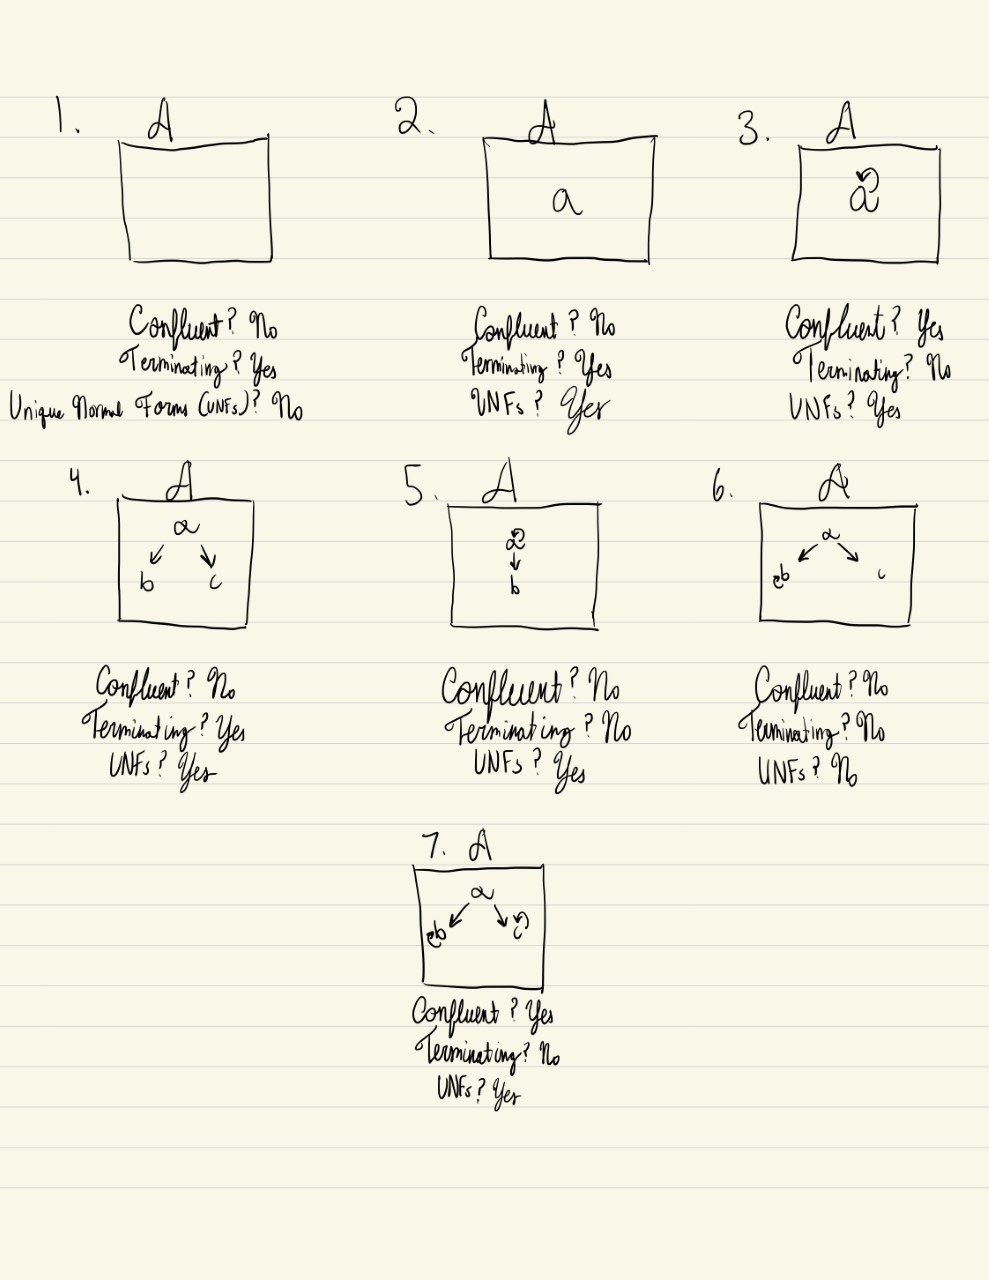
\includegraphics [scale=0.50]{ARS1}

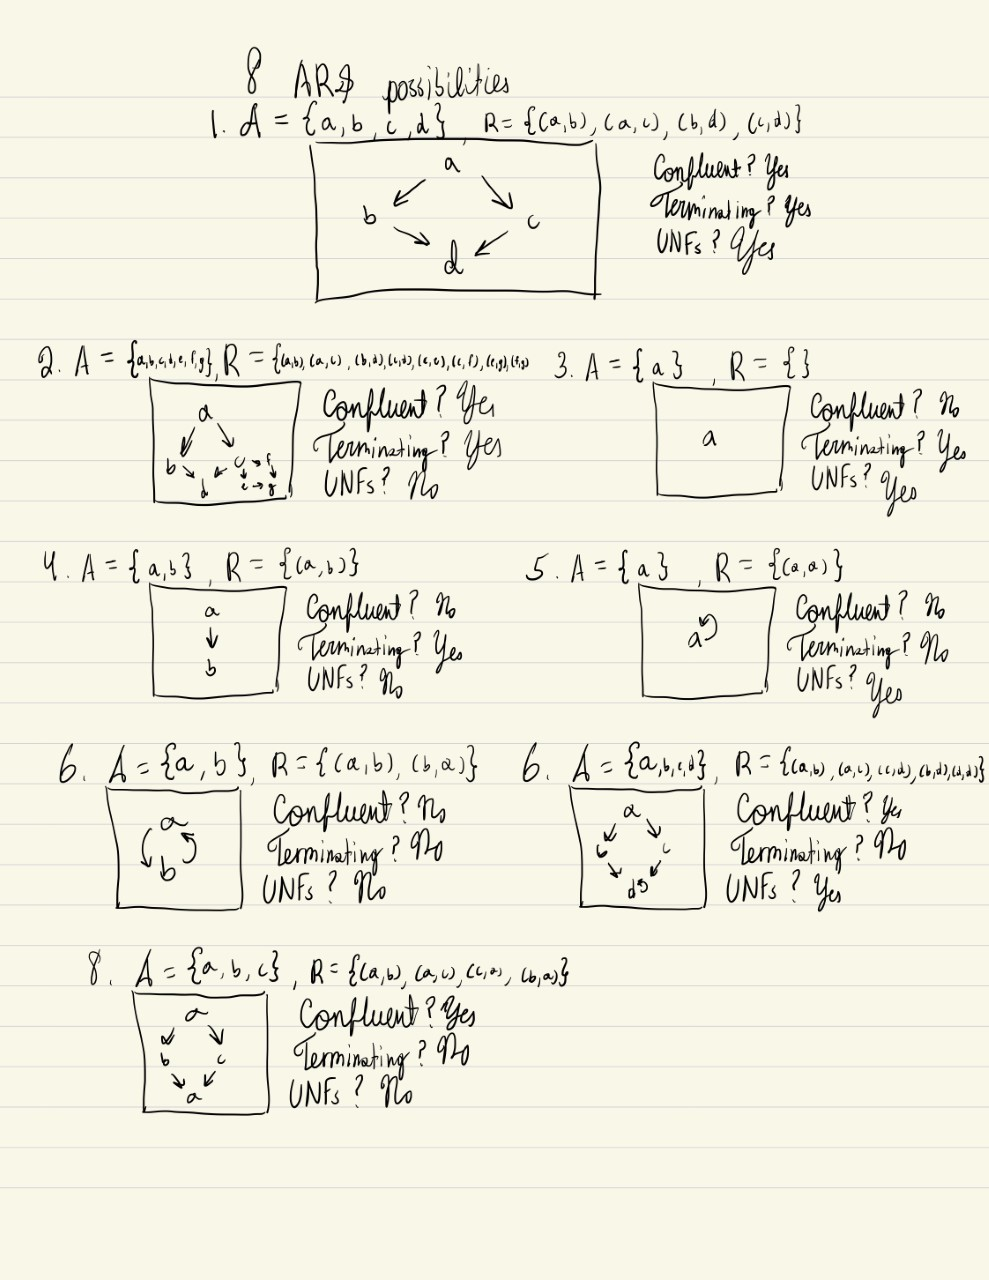
\includegraphics [scale=0.50]{ARS2}	

\subsection{Week 8}

1. The ARS does not terminate because the rewrite rules ba -> ab and ab -> ba allow for an infinite loop that doesn't terminate. There is no measure function for this ARS. 

2. The normal forms are an empty word, a, and b. 

3.We are unable to change this ARS to have unique normal forms while maintaining the same equivalence relations because the relation onf ba -> ab and ab -> ba remaining in the ARS do not allow for unique normal forms. 

4. The normal forms here mean that two of the same character are rewritten to just one of the characters and two different characters are rewritten in reverse order. This function could be used for taking the square root of numbers. This is because the square root of two numbers that are the same is just the number before they are multiplied together, and the square root of two different numbers multiplied together equals the square root of those two numbers multiplied together in reverse order.

\ldots

\section{Project}

Introductory remarks ...

The following structure should be suitable for most practical projects. 

\subsection{Specification}

For my course project, I intend to learn the basics of HTML and CSS, and JavaScript and use what I learn to create a portfolio of my projects, which I can use in job searches. The portfolio will use elements from both languages to make the website look and feel intuitive as well as aesthetically pleasing. I intend to recreate the calculator project to the best of my abilities from this course to test my understanding of the background needed to make the calculator as well as my understanding of JavaScript, HTML, and CSS. The website will contain multiple pages(such as a page for my resume, a page with all of my digital art projects, etc.) that the user can access via hyperlinks. The website will also contain a tutorial on the basics of HTML and CSS.

\subsection{Prototype}
\subsection{Documentation}
\subsection{Critical Appraisal}

\ldots

\section{Conclusions}\label{conclusions}

(approx 400 words)

In the conclusion, I want a critical reflection on the content of the course. Step back from the technical details. How does the course fit into the wider world of programming languages and software engineering?

\begin{thebibliography}{99}
\bibitem[PL]{PL} \href{https://github.com/alexhkurz/programming-languages-2022/blob/main/README.md}{Programming Languages 2022}, Chapman University, 2022.
\end{thebibliography}

\end{document}
